\documentclass[12pt]{article}
\usepackage[paper=letterpaper,margin=2cm]{geometry}
\usepackage{amsmath,amssymb,amsfonts}
\usepackage{newtxtext, newtxmath}
\usepackage{enumitem}
\usepackage{titling}
\usepackage[colorlinks=true]{hyperref}
\usepackage{multirow}
\usepackage{svg}
\usepackage{listings}
\usepackage{xcolor}
\usepackage{float}

\setlength{\droptitle}{-6em}

\definecolor{codegreen}{rgb}{0,0.6,0}
\definecolor{codegray}{rgb}{0.5,0.5,0.5}
\definecolor{codepurple}{rgb}{0.58,0,0.82}
\definecolor{backcolour}{rgb}{0.95,0.95,0.92}

\lstdefinestyle{mystyle}{
    commentstyle=\color{codegreen},
    keywordstyle=\color{magenta},
    numberstyle=\tiny\color{codegray},
    stringstyle=\color{codepurple},
    basicstyle=\ttfamily\footnotesize,
    breakatwhitespace=false,
    breaklines=true,
    captionpos=b,
    keepspaces=true,
    numbers=left,
    numbersep=5pt,
    showspaces=false,
    showstringspaces=false,
    showtabs=false,
    tabsize=2
}
\lstset{style=mystyle}

\begin{document}

\begin{center}
\large{Aprendizagem 2023}\\
Homework I -- Group 28\\
\vskip 0.3cm
Gonçalo Bárias (ist1103124) \& Raquel Braunschweig (ist1102624)\vskip 1cm

\large{\textbf{Part I}: Pen and Paper}\normalsize
\end{center}

\noindent Consider the partially learnt decision tree from the dataset $D$. $D$ is described by four input variables –
one numeric with values in $[0,1]$ and 3 categorical – and a target variable with three classes.

\begin{figure}[H]
    \centering
    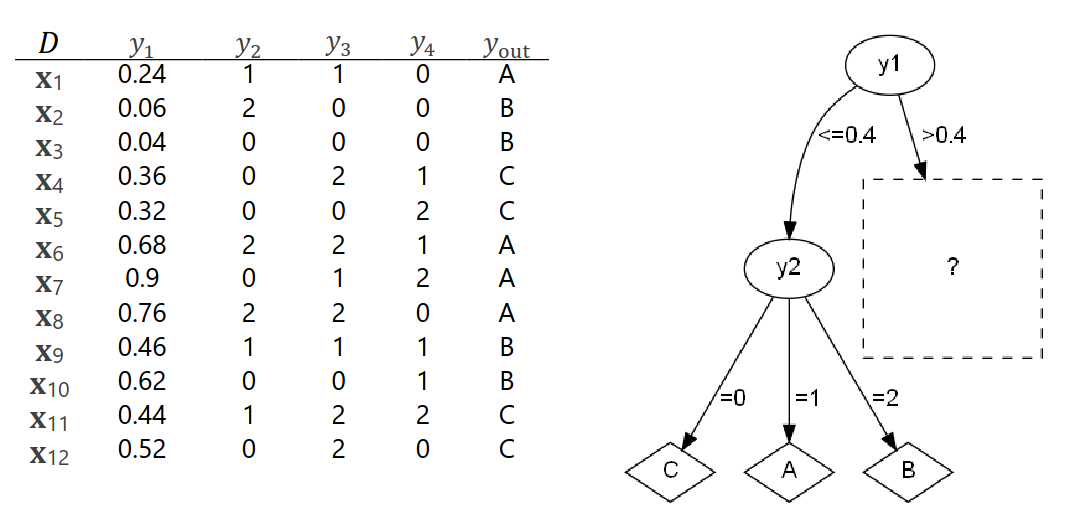
\includegraphics[width=15cm]{partial_tree_dataset_d}
    \caption{Partially Learnt Decision Tree and Dataset $D$ from Part I}
    \label{fig:PartI-partial-decision-tree-dataset-d}
\end{figure}

\begin{enumerate}[leftmargin=\labelsep]
    \item \textbf{Complete the given decision tree using Information gain with Shannon entropy ($log_2$).
    Consider that: i) a minimum of 4 observations is required to split an internal node, and
    ii) decisions by ascending alphabetic order should be placed in case of ties.}

    Blah

    \item \textbf{Draw the training confusion matrix for the learnt decision tree.}

    Blah

    \item \textbf{Identify which class has the lowest training F1 score.}

    Blah

    \item \textbf{Considering $y_2$ to be ordinal, assess if $y_1$ and $y_2$ are correlated using the Spearman coefficient.}

    Blah

    \item \textbf{Draw the class-conditional relative histograms of $y_1$ using 5 equally spaced bins in $[0,1]$.
    Find the root split using the discriminant rules from these empirical distributions.}

    Blah
\end{enumerate}

\vskip 0.5cm

\begin{center}
\large{\textbf{Part II}: Programming}\normalsize
\end{center}

\noindent Consider the \texttt{column\_diagnosis.arff} data available at the homework tab, comprising 6 biomechanical
features to classify 310 orthopaedic patients into 3 classes (\texttt{normal}, \texttt{disk hernia}, \texttt{spondilolysthesis}).

\begin{enumerate}[leftmargin=\labelsep]
    \item \textbf{Apply \texttt{f\_classif} from \texttt{sklearn} to assess the discriminative power of the input variables.
          Identify the input variable with the highest and lowest discriminative power.
          Plot the class-conditional probability density functions of these two input variables.}

          \vskip -0.5cm
          \begin{figure}[H]
              \centering
              \includesvg[width=14cm]{class_conditional_probability.svg}
              \caption{Class-conditional probability density functions of the highest and lowest discriminative power variables.}
              \label{fig:PartII-ex1-plot}
          \end{figure}

    \newpage
    \item \textbf{Using a stratified 70-30 training-testing split with a fixed seed (\texttt{random\_state=0}), assess in a
          single plot both the training and testing accuracies of a decision tree with depth limits in
          $\{1,2,3,4,5,6,8,10\}$ and the remaining parameters as default.\vskip 0.05cm
          \textit{[Optional]} Note that split thresholding of numeric variables in decision trees is non-deterministic
          in sklearn, hence you may opt to average the results using 10 runs per parameterization.}

          \vskip -0.5cm
          \begin{figure}[H]
              \centering
              \includesvg[width=14cm]{training_testing_accuracies.svg}
              \caption{Accuracy of trained decision tree, applied to both a test and training sets, for varying depth limits.}
              \label{fig:PartII-ex2-plot}
          \end{figure}

    \item \textbf{Comment on the results, including the generalization capacity across settings.}

          Blah

    \item \textbf{To deploy the predictor, a healthcare team opted to learn a single decision tree
          (\texttt{random\_state=0}) using \textit{all} available data as training data, and further ensuring that each leaf has
          a minimum of 20 individuals in order to avoid overfitting risks.}
          \begin{enumerate}
          \item \textbf{Plot the decision tree.}

          Blah

          \item \textbf{Characterize a hernia condition by identifying the hernia-conditional associations.}

          Blah
          \end{enumerate}
\end{enumerate}

\vskip 1cm
\center\textbf{END}

\end{document}
